\documentclass[a4paper, 12pt]{scrartcl}

\usepackage[english]{babel}
\usepackage[utf8]{inputenc}
\usepackage{csquotes}

% citations
\usepackage[
  natbib=true,
  backend=biber,
  doi=true,
  isbn=false,
  url=false,
  date=year,
  style=authoryear,
  citestyle=authoryear,
  minnames=1,
  maxnames=2,
  minbibnames=1,
  maxbibnames=99,
  uniquename=false,
  uniquelist=false]{biblatex}
\addbibresource{citramalate.bib}
\usepackage{varioref}

\usepackage{graphicx}
\graphicspath{ {./graphics/} }
\usepackage[font=small]{caption}
\usepackage[font=small]{subcaption}
\usepackage{url}
%\usepackage{varioref}
\usepackage{tabularx}
  \newcolumntype{L}{>{\raggedright\arraybackslash}X}
\usepackage[version=4]{mhchem}
\usepackage{siunitx}
\DeclareSIUnit\molar{\mole\per\cubic\deci\metre}
\DeclareSIUnit\Molar{\textsc{m}}
\DeclareSIUnit\calorie{cal}
\usepackage{booktabs}
\usepackage{longtable}
\usepackage{ltablex}
\usepackage{pgfplotstable}
\usepackage{tikz}
\usetikzlibrary{shapes,arrows}
\usepackage{physics}

\usepackage{setspace}


\begin{document}

  \title{Bridging the gap between stoichiometric and kinetic models to optimize the design of strains: the case study of citramalate production in \emph{E. coli}}

  \author{
    Arin Wongprommoon\\
    {\small Cambridge Systems Biology Centre, University of Cambridge, Cambridge, UK \thanks{
      Present address: Centre for Synthetic and Systems Biology, School of Biological Sciences, University of Edinburgh, Edinburgh, UK} } \and
    Jorge J\'ulvez \\
    {\small Cambridge Systems Biology Centre, University of Cambridge, Cambridge, UK \thanks{
      Present address: Department of Computer Science and Systems Engineering, University of Zaragoza, Zaragoza, Spain} } \and
    Stephen G Oliver\\
    {\small Cambridge Systems Biology Centre, University of Cambridge, Cambridge, UK }}

  \maketitle

  Running title: Insert one up to 45 characters here.

  \pagebreak

  \doublespacing
  
  \begin{abstract}

Genetically modified \emph{E. coli} can be used to synthesise chemicals of industrial interest. For example, strains possessing citramalate synthase can produce citramalate ((2\emph{S})-2-hydroxy-2-methylbutanedioate), a precursor for the production of plastics.
  This project used modelling approaches to find conditions that maximise the production of citramalate. The kinetic model described by \citet{millard_metabolic_2017} and the stoichiometric model described by \citet{orth_comprehensive_2011}, both for \emph{E. coli} metabolism, were extended by adding a reaction that produced citramalate from acetyl coenzyme A and pyruvate.
  
  Information from the kinetic model was used to enrich the stoichiometric model. The possible values of fluxes through each reaction were used to set the bounds for each reaction in the stoichiometric model. A strategy of mapping reactions between the kinetic model and the stoichiometric model was devised. Flux balance analysis (FBA) was then performed to evaluate the highest possible flux through the citramalate synthesis reaction as a proxy for citramalate productivity. This achieved an optimum solution of 0.2922 mM s\textsuperscript{-1}; however, a fork between citramalate production and growth was observed, which means that optimising both citramalate production and growth cannot be done using FBA alone. Flexible nets works... (insert content here).  Finally, composition of the Lund medium \citep{eastham_process_2015} was studied in an attempt to create bounds for relevant uptake reactions.

  \end{abstract}

  Keywords: insert, three, to, five, keywords, here

  \pagebreak
    
\section*{Introduction}
\label{sec:intro}

% GENERAL NOTES FOR WHOLE DRAFT
% - Write before editing (at this stage I'm mostly copy-pasting stuff from the extended report and moving stuff around)
% - Add data/appendices as supplementary information (or summarise the content in tables or figures) after I structure the main text.  This is pretty crucial, it's the data that drives the paper.
% - Obviously citations and justification needed, but these will come after the meat of the manuscript/draft
% - Make everything US spelling at the end (or at least settle on something consistent)

% Issue: using living organisms to synthesis chemicals is an alternative to fossil fuels; however, traditional wet-lab based methods to optimise such production is labourious.  Computational models can accelerate development, but currently two prevailing model types lack an interface that would make it much easier to optimise productivity.

Using living organisms to synthesise chemicals is an alternative to synthesising chemicals from fossil fuels, as it serves as a renewable resource with potentially high efficiency and low costs.  One such chemical is citramalate ((2\emph{S})-2-hydroxy-2-methylbutanedioate).  Citramalate is a chemical of industrial interest as it can be a precursor for methacrylic acid, a monomer for the production of plastics.  Citramalate synthesis is mediated by citramalate synthase (EC 2.3.1.182) in \emph{Methanococcus janaschii} \citep{wu_production_2016}, which catalyses the reaction:

\begin{center}
  acetyl-CoA + pyruvate + \ce{H2O} $\rightarrow$ CoA-SH + \ce{H^+} + citramalate
\end{center}

Traditional wet lab-based methods to optimise chemostat culture conditions for synthetic chemical production by microorganisms can be labourious.  Optimising culture conditions for production of chemicals such as citramalate can be accelerated by using mathematical models.  Currently, two prevailing mathematical model types that concern cellular metabolism are kinetic and stoichiometric models, which describe cellular metabolism from different points of view.

% Development of genome-scale models, kinetic, and stoichiometric models (cite key papers; they should also be cited by Millard et al., 2017 and Orth et al., 2011)

% Stoichiometric models contain more reactions but no information about reaction dynamics, and they can be enriched with information from kinetic models.  This is the novelty of the paper.

A stoichiometric model is a genome-scale reconstruction of the metabolic network of a model organism.  In contrast, a kinetic model only concerns central carbon metabolism, but contains initial conditions and substrate concentrations, which the stoichiometric model lacks. % This will obviously be longer and should cite key papers/reviews that define these two types of models
Neither model type alone is suited for the task of optimising productivity, and currently an interface between the two types of models is lacking.

% Case study is the Millard et al. (2017) kinetic model of central carbon metabolism in E. coli and the Orth et al. (2011) genome-scale stoichiometric model.  This is a description of the two models

This study concerns two models of \emph{E. coli} metabolism: a kinetic model described by \citet{millard_metabolic_2017} and a stoichiometric model described by \citet{orth_comprehensive_2011}.
  \emph{E. coli} was chosen as the model organism because its metabolism is well-characterised in mathematical models, because predictions from models can be verified in cultures that are easy to maintain, and because there are \emph{E. coli} strains that have been genetically engineered to produce citramalate.
  This enzyme is not present in wild-type \emph{E. coli} strains, so in experiments \emph{E. coli} is engineered to express the \emph{cimA} gene that encodes citramalate synthase \citep{wu_production_2016}.
The kinetic model contains 68 reactions, 49 of which include $V_{max}$ as a parameter.  The $V_{max]$ value is relevant because according to Michaelis-Menten kinetics, enzyme activity is proportional to $V_{max}$ and this relation can be easily exploited in engineering \emph{E. coli} to optimise citramalate production.  Of these reactions, 41 correspond to real enzyme-catalysed reactions.  The stoichiometric model contains 2,584 reactions, most of which do not have flux boundaries by default.

% Aims: Here I'm developing a method to map reactions between the two models, and then using simulations in the kinetic model to accordingly set fluxes in the stoichiometric model.  Ultimately this leads to non-linear optimisation of the production of citramalate.

This study aims to bridge the gap between the kinetic and stoichiometric models by devising a method of map reactions between the two models, and by using simulations in the kinetic model to set fluxes in the stoichiometric model.  This study also shows that the flexible nets formalism can be used to solve a non-linear optimisation problem that aims to optimise both growth and citramalate productivity based on the enriched stoichiometric model, supplanting the use of flux balance analysis.

% \begin{enumerate}
% \item Investigating how $V_{max}$ values of reactions in the kinetic model affect citramalate productivity, and finding a method to find such values that would optimise citramalate productivity;
% \item Bridging the gap between the kinetic and stoichiometric models, by using simulations in the kinetic model to set fluxes in the stoichiometric model, and by devising a method of map reactions between the two models; and
%   \item Using information from the Lund medium \citep{eastham_process_2015} on the models to determine how nutrient medium composition affects citramalate productivity, and investigating how this information can be used to improve the Lund medium.
%   \end{enumerate}


% This strategy can be generalised and applied to other models.
The strategies used in this study may be applied to other pairs of kinetic and stoichiomentric models that are related to each other, and may be expanded to solve other optimisation problems.

  
\section*{Materials and Methods}
\label{sec:methods}

Insert text here.

To investigate citramalate production, a 69th reaction called CITRA\_SYN was added to the kinetic model to model citramalate synthesis.  In the model, this reaction has the Michaelis-Menten kinetic law:

\begin{equation}
  \frac{\mathrm{d}[citramalate]}{\mathrm{d}t} = 
  \frac{V_{max} \cdot [acetyl-CoA]}{[acetyl-CoA] + K_{m}}
\end{equation}
\label{eq:michaelismenten}

This kinetic law assumes that pyruvate is saturating. $V_{max}$ is set to 4 mM s\textsuperscript{-1} and $K_{m}$ to 0.495 mM in the modified model. These values are based on experimental values obtained in the ConBioChem project.

Manipulating the SBML file encoding the kinetic model required the Python library \texttt{libsbml} \citep{bornstein_libsbml:_2008} and running simulations employed the \texttt{roadrunner} \citep{somogyi_libroadrunner:_2015} module. The simulations ran from 0 to 7,200 seconds, at which steady-state was attained for almost all conditions.
Using this modified kinetic model, I investigated the effect of parameters on citramalate productivity. Citramalate productivity is defined as $\mu \cdot Y_{P/S}$, where $\mu$ is the growth rate in reciprocal time units (h\textsuperscript{-1}) and $Y_{P/S}$ is defined as the mass of the product (citramalate) divided by the mass of the substrate (glucose).

A 2,585th reaction for citramalate production was added to the stoichiometric model using the \texttt{cobra} module \citep{ebrahim_cobrapy:_2013} in Python. This reaction contains the same information as the reaction added to the kinetic model except for the kinetic law, which is normally absent from stoichiometric models. In addition, a sink reaction to allow citramalate to leave the system was also added.
Fluxes through reactions in the stoichiometric model were investigated using flux balance analysis, or FBA \citep{orth_what_2010}, and FBA simulations employed the \texttt{cobra} module.

% [This might be more appropriate in the discussion; it is an important part of the project and it does relate the two models, but it seems out of place in an otherwise `expository' introduction. If this is moved to the discussion, I might comment on using different values for the ratio between cell dry weight and cell volume, but I honestly don't think it's important enough to deserve a mention]
The kinetic and stoichiometric models use different units. Fluxes are in mM s\textsuperscript{-1} in the kinetic model, but are mmol g\textsubscript{DW}\textsuperscript{-1} h\textsuperscript{-1} in the stoichiometric model. Using the cell volume of \num{1.77e-3} L g\textsubscript{DW}\textsuperscript{-1} as specified in the kinetic model, I worked out that converting values from the kinetic model to the stoichiometric model involves multiplying by 6.372\footnote{
($R$ mM s\textsuperscript{-1})(\num{1.77e-3} L g\textsubscript{DW}\textsuperscript{-1})(3600 s h\textsuperscript{-1}) = 6.372 $R$ mmol g\textsubscript{DW}\textsuperscript{-1} h\textsuperscript{-1}
}.
% [I am not sure about this -- there may be the issue that the stoichiometric model is not tuned for small flux values]
%Because the stoichiometric model does not have information about enzyme kinetics, the values associated with the kinetic model (with kinetic model units) can be used with the structure of the stoichiometric model without any adjustments.

\section*{Modeling or Theoretical Aspects}
\label{sec:theory}

Insert text here.  This is an optional section.  Note US spelling of heading.

\section*{Results}
\label{sec:results}

Insert text here.

\subsection*{Enhancing a genome-scale stoichiometric model with information from a kinetic model}
\label{ssec:results-enhance}

The stoichiometric model can be enhanced by applying flux boundaries that are derived from reaction fluxes attained in kinetic model simulations.  In order to do that, an adequate strategy to map reactions between a kinetic model and a stoichiometric model developed by different authors must be developed.

We developed a mapping table between the stoichiometric model and the kinetic model that
concerns the 68 reactions present in the wild-type kinetic model, including the growth reaction. The full mapping table included:
\begin{itemize}
\item Kinetic and stoichiometric model reaction IDs and stoichiometries, plus stoichiometric model reaction names
  \item EC numbers for kinetic model reactions quoted by \citet{millard_metabolic_2017} and EC number for stoichiometric model reactions extracted from the respective SBML file
\item Categorisation of reactions into sub-systems as specified by \citet{millard_metabolic_2017}
  \item Relationships and differences between stoichiometric model reactions and the corresponding kinetic model reactions
\end{itemize}

Three reactions are absent in the stoichiometric model (GL6P\_HYDROLYSIS, ACEK\_1, and ACEK\_2), so the fluxes of these reactions were ignored in the mapping. Additionally, stoichiometric CYTBO3\_4pp has a different stoichiometry from kinetic CYTBO. Furthermore, the growth reactions from the two models use different coefficients.

Fifteen reactions are identical between the kinetic and stoichiometric model. Reactions that are not identical fall into the following categories:

\begin{enumerate}
\item \emph{Plus small chemical species:} reactions that are otherwise identical, but differ by the addition of the species \ce{H^+} or \ce{H2O}
\item \emph{Acid hydrolysis:} reactions that are otherwise identical, but \ce{CO2} is listed in the stoichiometric model in place of \ce{HCO3^-}
\item \emph{Different reversibility:} reactions that are otherwise identical, but are reversible in the stoichiometric model with its counterpart in the kinetic model being irreversible, or vice versa
\item \emph{Reversed:} reactions that are reversed with respect to one another
  \item \emph{Sub-network different structure:} reactions that belong to sub-networks that are structured differently and therefore do not allow one-to-one mapping; these include the glucose uptake and the pentose phosphate pathway sub-systems
  \end{enumerate}

I devised rules to map flux values from the kinetic model onto the stoichiometric model. For categories 1--3, stoichiometric model reactions have the same lower and upper flux bounds as their kinetic model counterparts. For category 4, the values were negated: i.e. $ \mathrm{Kinetic } (LB, UB) \rightarrow \mathrm{Stoichiometric } (-UB, -LB)$. %note: might need overfull hbox fixes/bodges depending on how this looks like in the final version

Reactions in category 5 demanded special treatment. Their architectures in the two models are summarised in figures~\ref{fig:glucoseuptake} and~\ref{fig:ppp}.

\begin{figure}[!p]
  \centering
  \includegraphics[scale=0.4]{glucoseuptake}
  \caption{Sub-network for glucose uptake}
  \label{fig:glucoseuptake}
\end{figure}

\begin{figure}[!p]
  \centering
  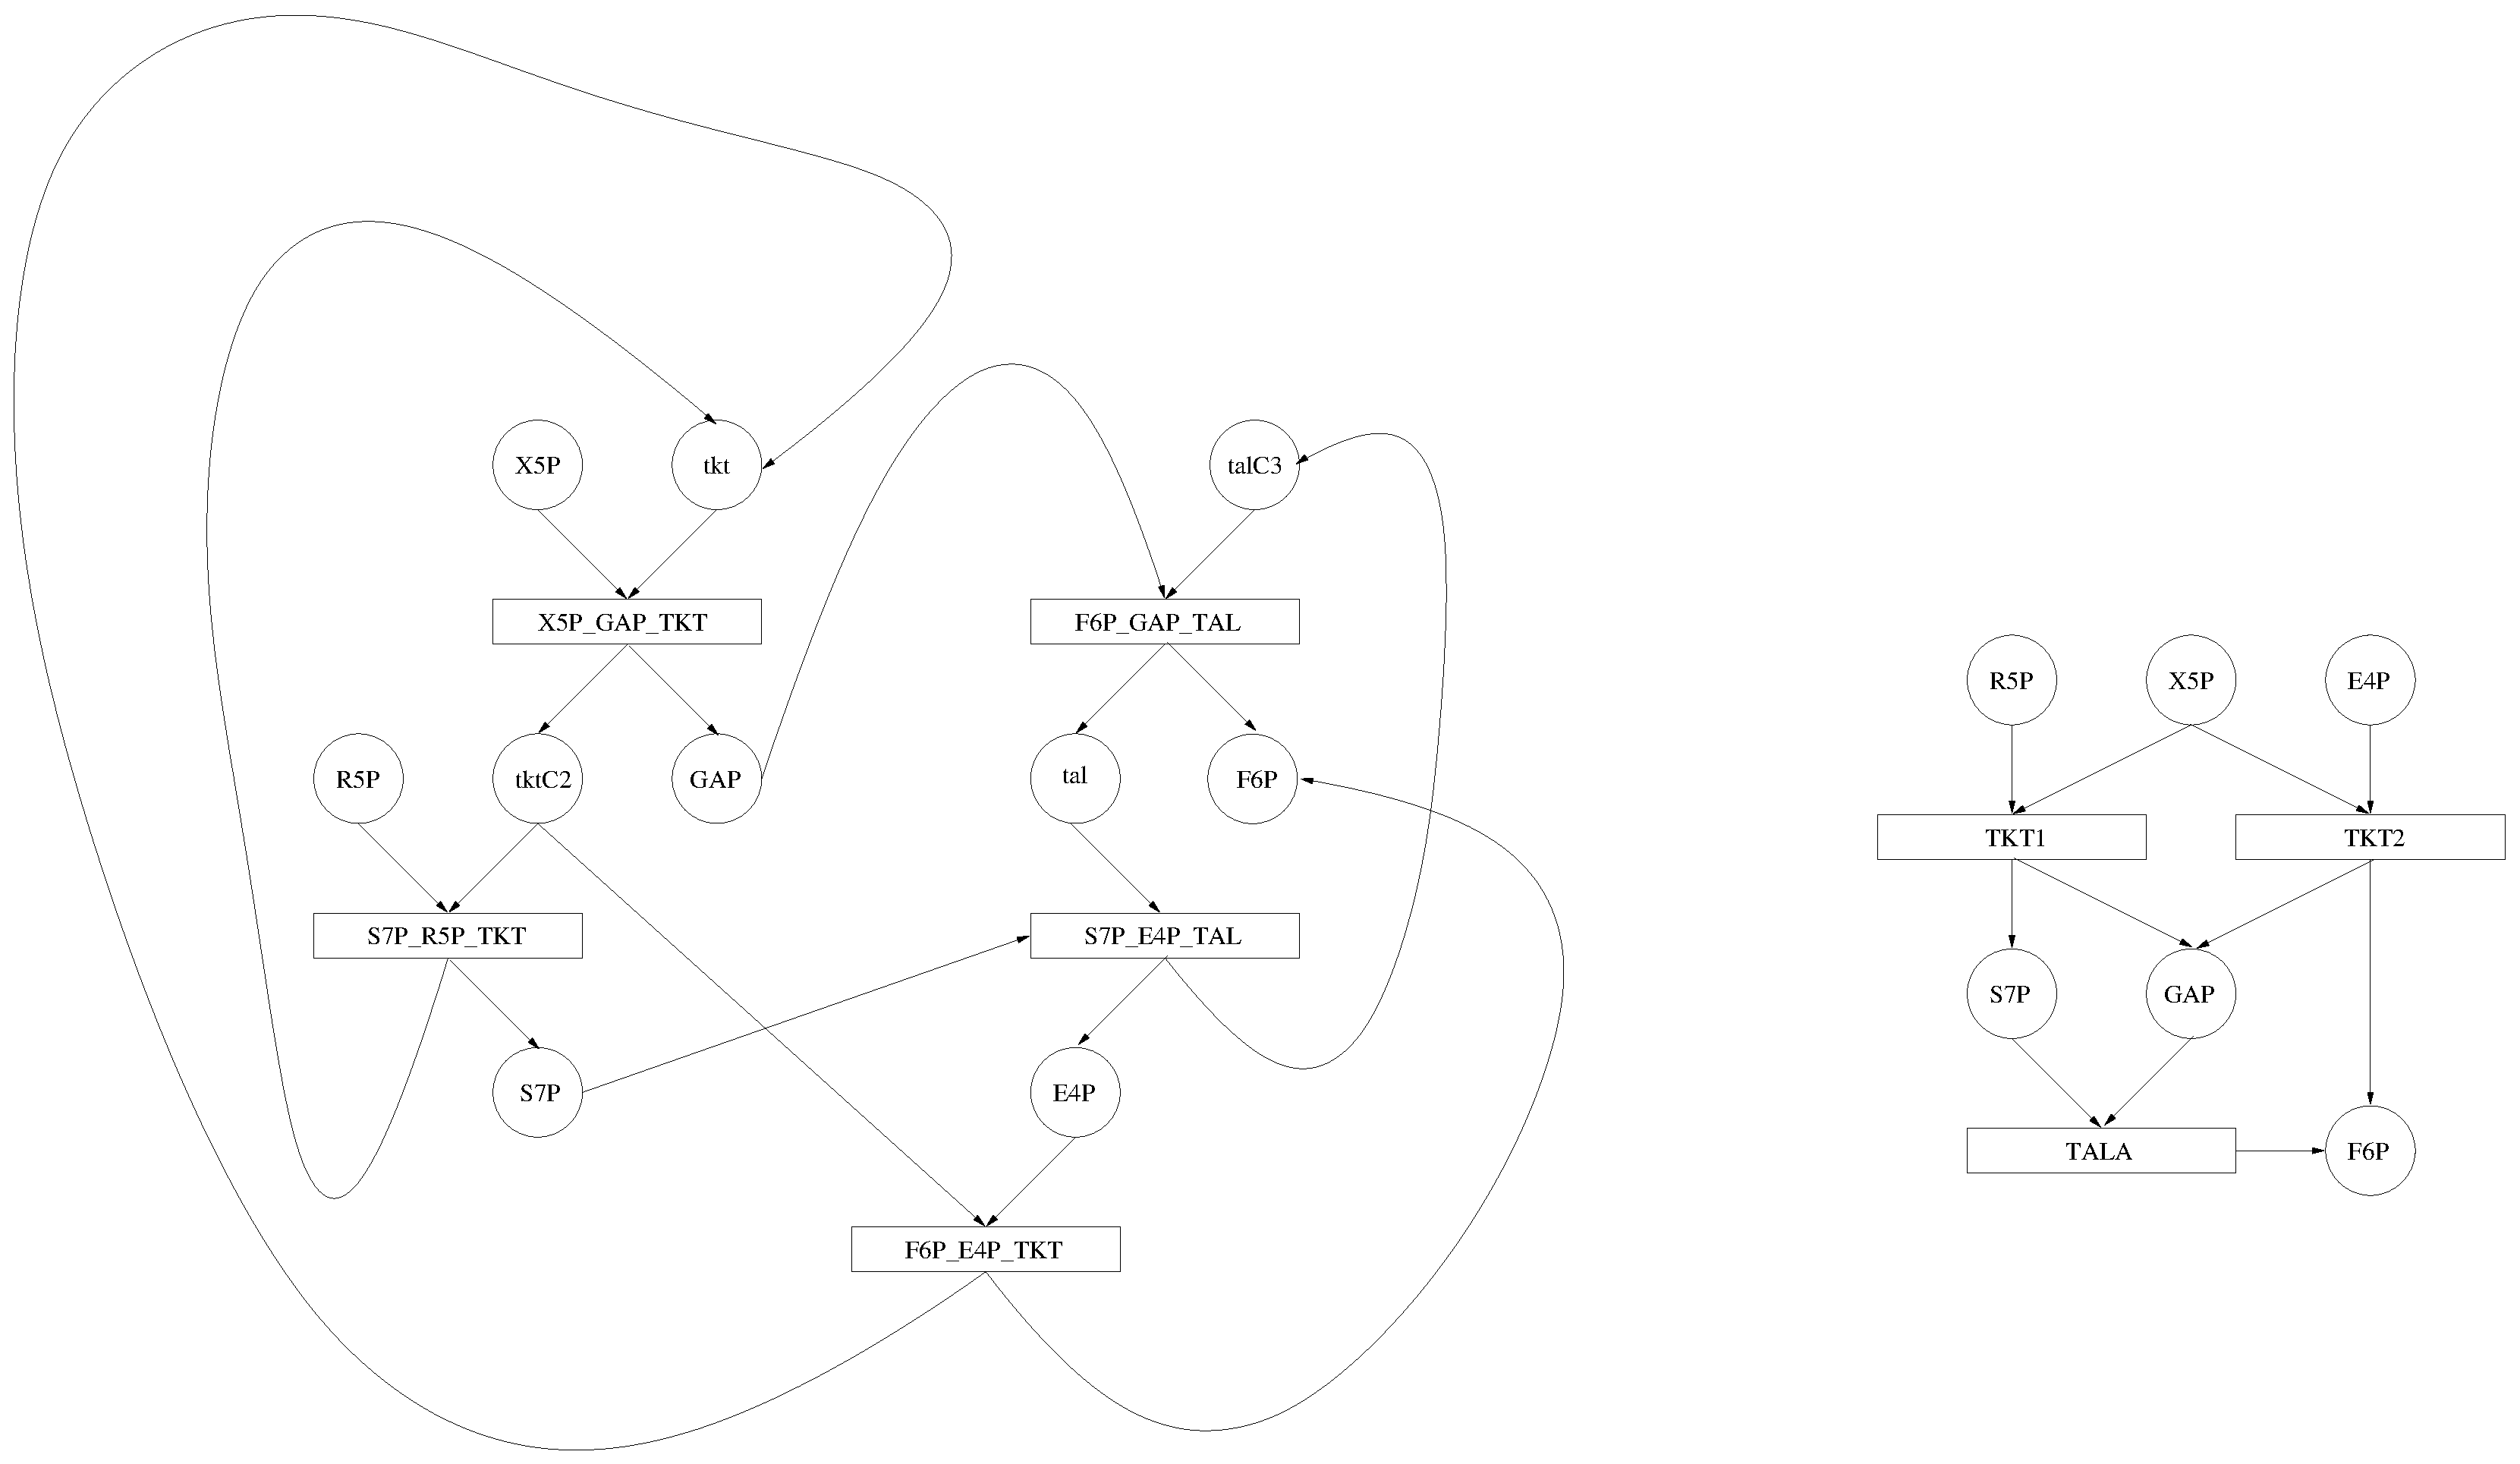
\includegraphics[scale=0.25]{ppp}
  \caption{Sub-network for part of the pentose phosphate pathway; left - kinetic model, right - stoichiometric model}
  \label{fig:ppp}
\end{figure}

I mapped glucose uptake reactions according to table~\ref{tab:glucoseuptake}. Mapping GLC\_feed to EX\_glc\_(e) is based on how both correspond to glucose feed into the environment, and mapping XCH\_GLC to GLCtex is based on the species involved on both sides of the reaction. However, mapping PTS\_0 to PTS\_4 to GLCptspp is based on investigating their behaviour in response to varying flux through GLC\_feed.

\begin{table}[!htbp]
  \caption{Mapping glucose uptake reactions}
  \label{tab:glucoseuptake}
  \centering
  \begin{tabularx}{\linewidth}{LLL}
    \toprule
    Kinetic model & Stoichiometric model & What it is\\
    \midrule
    GLC\_feed & EX\_glc\_(e) & Glucose feed (chemostat) into the environment\\
    XCH\_GLC & GLCtex & Glucose transport from environment to periplasm\\
    PTS\_0, PTS\_1, PTS\_2, PTS\_3, PTS\_4 & GLCptspp & Glucose uptake from periplam to cytoplasm\\
    \bottomrule
  \end{tabularx}
\end{table}

For the pentose phosphate pathway reactions, I focussed on each metabolite (X5P, GAP, R5P, S7P, F6P, and E4P) separately to determine the influx reactions (that produce the metabolite) and the efflux reactions (that consume the metabolite). I based the mapping on the principle that the sum of influxes in the kinetic model must be equivalent to the sum of influxes in the stoichiometric model, and that the same holds for effluxes (figure~\ref{fig:pppmapping}).

\tikzstyle{met} = [draw, circle]
\tikzstyle{reac} = [rectangle]
\tikzstyle{line} = [draw, -latex']

\begin{figure}[h]
  \centering
  \begin{tikzpicture}[node distance = 1.5cm, every node/.style={scale=0.8}]
    % stoichiometric model metabolites
    \node [reac] (stolabel) {Stoichiometric model};
    \node [met, below of=stolabel] (x5psto) {X5P};
    \node [met, below of=x5psto] (gapsto) {GAP};
    \node [met, below of=gapsto] (r5psto) {R5P};
    \node [met, below of=r5psto] (s7psto) {S7P};
    \node [met, below of=s7psto] (f6psto) {F6P};
    \node [met, below of=f6psto] (e4psto) {E4P};
    %stoichiometric model reactions and arrows
    \node [reac, right of=x5psto, xshift=1.25cm] (x5psto-x5pgaptkt) {X5P\_GAP\_TKT};
    \path [line] (x5psto) -- (x5psto-x5pgaptkt);

    \node [reac, left of=gapsto, xshift=-1.25cm] (gapsto-x5pgaptkt) {X5P\_GAP\_TKT};
    \path [line] (gapsto-x5pgaptkt) -- (gapsto);    
    \node [reac, right of=gapsto, xshift=1.25cm] (gapsto-f6pgaptal) {F6P\_GAP\_TAL};
    \path [line] (gapsto) -- (gapsto-f6pgaptal);

    \node [reac, right of=r5psto, xshift=1.25cm] (r5psto-s7pr5ptkt) {S7P\_R5P\_TKT};
    \path [line] (r5psto) -- (r5psto-s7pr5ptkt);

    \node [reac, left of=s7psto, xshift=-1.25cm] (s7psto-s7pr5ptkt) {S7P\_R5P\_TKT};
    \path [line] (s7psto-s7pr5ptkt) -- (s7psto);    
    \node [reac, right of=s7psto, xshift=1.25cm] (s7psto-s7pe4ptal) {S7P\_E4P\_TAL};
    \path [line] (s7psto) -- (s7psto-s7pe4ptal);

    \node [reac, left of=f6psto, xshift=-1.25cm, yshift=0.25cm] (f6psto-f6pgaptal) {F6P\_GAP\_TAL};
    \node [reac, left of=f6psto, xshift=-1.25cm, yshift=-0.25cm] (f6psto-f6pe4ptkt) {F6P\_E4P\_TKT};
    \path [line] (f6psto-f6pgaptal) -- (f6psto);
    \path [line] (f6psto-f6pe4ptkt) -- (f6psto);    

    \node [reac, left of=e4psto, xshift=-1.25cm] (e4psto-s7pe4ptal) {S7P\_E4P\_TAL};
    \path [line] (e4psto-s7pe4ptal) -- (e4psto);    
    \node [reac, right of=e4psto, xshift=1.25cm] (e4psto-f6pe4ptkt) {F6P\_E4P\_TKT};
    \path [line] (e4psto) -- (e4psto-f6pe4ptkt);

    %kinetic model metabolites
    \node [reac, right of=stolabel, xshift=6cm] (kinlabel) {Kinetic model};
    \node [met, below of=kinlabel] (x5pkin) {X5P};
    \node [met, below of=x5pkin] (gapkin) {GAP};
    \node [met, below of=gapkin] (r5pkin) {R5P};
    \node [met, below of=r5pkin] (s7pkin) {S7P};
    \node [met, below of=s7pkin] (f6pkin) {F6P};
    \node [met, below of=f6pkin] (e4pkin) {E4P};
    %kinetic model reactions and arrows
    \node [reac, right of=x5pkin, xshift=0.5cm, yshift=0.25cm] (x5pkin-tkt1) {TKT1};
    \node [reac, right of=x5pkin, xshift=0.5cm, yshift=-0.25cm] (x5pkin-tkt2) {TKT2};
    \path [line] (x5pkin) -- (x5pkin-tkt1);
    \path [line] (x5pkin) -- (x5pkin-tkt2);

    \node [reac, left of=gapkin, xshift=-0.5cm, yshift=0.25cm] (gapkin-tkt1) {TKT1};
    \node [reac, left of=gapkin, xshift=-0.5cm, yshift=-0.25cm] (gapkin-tkt2) {TKT2};
    \node [reac, right of=gapkin, xshift=0.5cm] (gapkin-tala) {TALA};
    \path [line] (gapkin-tkt1) -- (gapkin);
    \path [line] (gapkin-tkt2) -- (gapkin);
    \path [line] (gapkin) -- (gapkin-tala);

    \node [reac, right of=r5pkin, xshift=0.5cm] (r5pkin-tkt1) {TKT1};
    \path [line] (r5pkin) -- (r5pkin-tkt1);

    \node [reac, left of=s7pkin, xshift=-0.5cm] (s7pkin-tkt1) {TKT1};
    \path [line] (s7pkin-tkt1) -- (s7pkin);    
    \node [reac, right of=s7pkin, xshift=0.5cm] (s7pkin-tala) {TALA};
    \path [line] (s7pkin) -- (s7pkin-tala);

    \node [reac, left of=f6pkin, xshift=-0.5cm, yshift=0.25cm] (f6pkin-tala) {TALA};
    \node [reac, left of=f6pkin, xshift=-0.5cm, yshift=-0.25cm] (f6pkin-tkt2) {TKT2};
    \path [line] (f6pkin-tala) -- (f6pkin);
    \path [line] (f6pkin-tkt2) -- (f6pkin);    

    \node [reac, left of=e4pkin, xshift=-0.5cm] (e4pkin-tala) {TALA};
    \path [line] (e4pkin-tala) -- (e4pkin);    
    \node [reac, right of=e4pkin, xshift=0.5cm] (e4pkin-tkt2) {TKT2};
    \path [line] (e4pkin) -- (e4pkin-tkt2);

  \end{tikzpicture}
  \caption{Rationale for mapping pentose phosphate pathways reactions between the kinetic and stoichiometric models}
  \label{fig:pppmapping}
\end{figure}


As a result, I produced the following rules:
\begin{itemize}
\item Kinetic X5P\_GAP\_TKT = Stoich.\ TKT1 + Stoich.\ TKT2 (from focussing on X5P and on GAP)
\item Kinetic F6P\_GAP\_TAL = Stoich.\ TALA (from focussing on GAP and on F6P)
\item Kinetic S7P\_R5P\_TKT = Stoich.\ TKT1 (from focussing on R5P and on S7P)
\item Kinetic S7P\_E4P\_TAL = Stoich.\ TALA (from focussing on S7P and on E4P)
  \item Kinetic F6P\_E4P\_TKT = Stoich.\ TKT2 (from focussing on F6P and on E4P)
  \end{itemize}

  This means that the lower bound of the sum of the fluxes of stoichiometric model TKT1 and stoichiometric model TKT2 is equal to the lower bound of kinetic model X5P\_GAP\_TKT, and the same applies to the upper bound. For the other reactions, the lower bound of the kinetic model reaction is equal to the upper bound of the corresponding stoichiometric model reaction, and the same applies to the upper bound.

  The strategies described can be generalised to other pairs of stoichiometric and kinetic models that are related to each other.

\subsection*{Kinetic model simulations can be used to define flux bounds for the stoichiometric model}
\label{ssec:results-bounds}

The stoichiometric model consists of reaction stoichiometries along with lower and upper bounds for flux for each reaction. These bounds can be specified to provide constraints for FBA.
The lowest and highest possible values of fluxes through each reaction in the kinetic model provides reasonable bounds for the stoichiometric model.
To find the lowest and highest possible flux values through the 69 reactions of the kinetic model, I varied the $V_{max}$ values of the 49 reactions with $V_{max}$ as a parameter, CITRA\_SYN included.

Initially, to save computation time, I varied $V_{max}$ values of one reaction at a time over the range of 0.1-10.0 $V_{max}$, and recorded the minimum and maximum flux values achieved for each reaction after simulations. These produced a set of flux bounds I term `one-dimension bounds' (data not shown).
I then investigated the sensitivity of such bounds when the $V_{max}$ range was changed. The smaller the $V_{max}$ range over which the one-dimension flux bounds were generated, the lower the difference between the computed upper and lower bounds.  Additionally, the sum of differences among all reactions seemed to plateau beyond 5.0 $V_{max}$ (figure~\ref{fig:vmaxplateau})

\begin{figure}[h]
  \centering
  \includegraphics[scale=0.3]{vmaxplateau}
  \caption{Relationship between $V_{max}$ ranges used for generating one-dimension flux bounds and the sum of differences between upper and lower bounds for each reaction}
  \label{fig:vmaxplateau}
\end{figure}

Then, I used differential evolution to find the lowest and highest possible fluxes through each kinetic model reaction. The simulated flux through each reaction was the objective function. To calculate the lower bound for each reaction, this objective function was minimised, and to calculate the upper bound, it was maximised.

First, I included the eight reactions with the greatest flux control coefficients: CYTBO, MQO, MDH, ZWF, GLT, GDH, ATP\_syn, and ACK, with parameters $F$ = 0.6607, $CR$ = 0.9426, $NP$ = 28, and 5 iterations \citep{pedersen_good_2010}. I used the $V_{max}$ range of of 0.3--10.0 $V_{max}$ because $V_{max}$ values less than 0.3 $V_{max}$ tended to produce run time errors in \texttt{roadrunner}, in which convergence test failures occurred too many times. Using this restricted range was justified by the aberrant behaviour of ATP\_MAINTENANCE (section~\ref{sec:couples}), which suggested that the model was not reliable with such small $V_{max}$ values. From this work, I produced `eight-dimension bounds' (data not shown). Increasing the number of iterations to 20 only marginally broadened the bounds.

Second, I included all 41 enzyme-catalysed reactions in the kinetic model with $V_{max}$ as a parameter. Here, I used the differential evolution parameters of $F$ = 0.6876, $CR$ = 0.9784, $NP$ = 48 \citep{pedersen_good_2010}, and five iterations. To avoid convergence test failures, I set the $V_{max}$ range to 0.5--10.0 $V_{max}$. From this, I produced `41-dimension bounds' (appendix~\ref{ap:41dbounds}).

The 41-dimension bounds were mostly wider than both one- and eight-dimension bounds. 41-dimension lower bounds were the most negative among the three sets for 43 of 57 reactions, and 41-dimension upper bounds were the most positive for 42 out of 57 reactions.

I performed FBA to test how flux information from the kinetic model can enrich the stoichiometric model in restricting reaction fluxes.
Using the mapping rules described in section~\ref{sec:mapping}, I prepared bounds for FBA from the kinetic model flux values obtained in section~\ref{sec:bounds}. Setting the objective to maximising to flux through the citramalate flux reaction, I obtained the results in table~\ref{tab:citramalatefluxresults}.

\begin{table}[!htbp]
  \caption{FBA results using citramalate flux as the objective function}
  \label{tab:citramalatefluxresults}
  \centering
  \begin{tabular}{lS}
    \toprule
    Bounds & \multicolumn{1}{c}{Solution (mM s\textsuperscript{-1})}\\
    \midrule
    Default & 1.9479\\ % Changed from 12.4122. I believe that number was using standard stoichiometric model units, but numbers below use bounds directly from the kinetic model without considering the 6.372 conversion factor. Just to make the units consistent
    Anargyros's & 0.3067\\
    Varying one reaction at a time & 0.2599\\
    Differential evolution with 8 reactions & 0.1925\\
    Differential evolution with 41 reactions & 0.2922\\
    \bottomrule
  \end{tabular}
\end{table}

% NEW: FBA failing on growth
However, FBA applied on the stoichiometric model using default bounds predicted zero growth if citramalate flux is maximised and predicts zero citramalate flux if growth is maximised. In other words, the solution of FBA diverts all the incoming flux either towards growth or towards citramalate production, depending on the objective function. As the stoichiometric model does not incorporate concentrations of chemical species, there is no way to find out citramalate productivity from the stoichiometric model.

\subsection*{Flexible nets can be used to optimise growth and productivity}
\label{ssec:results-fn}

Here, we converted the SBML model that encodes the enriched stoichiometric model to the flexible net formalism so that a nonlinear function can be optimised, namely optimising growth \emph{and} productivity.

% The Lund medium bit can be MUCH shorter and potentially come AFTER the part where I (hopefully) demonstrate that flexible nets work.  It will demonstrate that citramalate production can be optimised for media composition, thus completing the narrative.

(The flexible nets content should be here)

To test the optimisation, I investigated how to use the composition of a fermentation medium to inform the choice of flux bounds for the stoichiometric model. The aim was to improve the recipe of the medium to optimise citramalate production, based on how the model predicted fluxes for exchange reactions involving specific chemical species.

The patent WO 2015/022496 \citep{eastham_process_2015} describes a fermentation medium on p.79, for \emph{E. coli} BW25113 $\Delta$\emph{pflB} $\Delta$\emph{ldhA} transformed with pBAD24-\emph{cimA} to optimise production of (\emph{R})-citramalic acid:

\begin{center}
\begin{tabular}{lSr}
  Glucose & 11.9 & g L\textsuperscript{-1}\\
  \ce{(NH4)2SO4} & 2 & g L\textsuperscript{-1}\\
  \ce{K2HPO4} & 14.6 & g L\textsuperscript{-1}\\
  \ce{NaH2PO4.2H2O} & 3.6 & g L\textsuperscript{-1}\\
  \ce{(NH4)2H} citrate & 0.5 & g L\textsuperscript{-1}\\
  \ce{MgSO4} & 0.24 & g L\textsuperscript{-1}\\
  \ce{CaCl2.2H2O} & 1 & mg L\textsuperscript{-1}\\
  \ce{FeCl3} & 20.06 & mg L\textsuperscript{-1}\\
  \ce{ZnSO4.7H2O} & 0.36 & mg L\textsuperscript{-1}\\
  \ce{CuSO4.5H2O} & 0.32 & mg L\textsuperscript{-1}\\
  \ce{MnSO4.H2O} & 0.30 & mg L\textsuperscript{-1}\\
  \ce{CoCl2.6H2O} & 0.36 & mg L\textsuperscript{-1}\\
  \ce{Na2EDTA.2H2O} & 44.6 & mg L\textsuperscript{-1}                             
\end{tabular}
\end{center}

This is the `Lund medium' in this project.  Each chemical species is present in the following amounts:

\begin{center}
\begin{tabular}{lS}
  Species & \multicolumn{1}{c}{Concentration (mM)}\\
  \midrule
  \ce{K^{+}} & 167.6\\
  phosphates & 106.9\\
  glucose & 66.05\\
  \ce{NH4^+} & 34.69\\
  \ce{Na^+} & 23.32\\
  \ce{SO4^{2-}} & 17.13\\
  \ce{Hcitrate} & 2.211\\
  \ce{Mg^{2+}} & 1.994\\
  \ce{Cl^-} & 0.3876\\
  \ce{Fe^{3+}} & 0.1237\\
  EDTA & 0.1198\\
  \ce{Ca^{2+}} & 0.006802\\
  \ce{Mn^{2}+} & 0.001775\\
  \ce{Co^{2}+} & 0.001513\\
  \ce{Cu^{2+}} & 0.001282\\
  \ce{Zn^{2+}} & 0.001252\\
\end{tabular}
\end{center}

To conform to the exchange reactions defined in the stoichiometric model, \ce{HPO4^{2-}} and \ce{H2PO4^-} were merged into one entry representing inorganic phosphates. The stoichiometric model lacks an exchange reaction for EDTA, so this species was ignored in subsequent investigations.

In order to use the concentrations of the species present in the Lund medium to set the bounds of exchange reactions, additional information is needed.
\citet{chassagnole_dynamic_2002} concern the development of a dynamic model that links the sugar transport system of \emph{E. coli} with glycolysis and the pentose phosphate pathway.  Their study utilises growth conditions consistent with the model by \citet{millard_metabolic_2017}: \SI{37}{\celsius}, pH 7.0, steady-state conditions, and a dilution rate ($D$) of \SI{0.1}{\per\hour}.  The medium used includes \SI{20.0}{\gram\per\litre} glucose.

The study presents a model concerning glucose uptake:

\begin{equation}
  \dv{C_{glc}^{ext}}{t} = D(C_{glc}^{feed} - C_{glc}^{ext}) + f_{pulse} - \frac{C_{x}r_{PTS}}{\rho_{x}}
\end{equation}
\label{eqn:chassagnole_orig}

Where:

\begin{itemize}
\item $D$ is the dilution rate, \SI{0.1}{\per\hour} in this study, equal to that of the kinetic model
\item $C_{glc}^{feed}$ is the concentration of glucose in the medium fed to the continuous culture, \SI{20.0}{\gram\per\litre} in this study
\item $C_{glc}^{ext}$ is the external concentration of glucose in the chemostat, measured to be \SI{0.0556}{\milli\Molar} in this study
\item $f_{pulse}$ is a variable that accounts for the sudden change of glucose concentration caused by the glucose pulse experiments in the study
\item $C_{x}$ is the biomass concentration, measured to be 8.7 g\textsubscript{DW} bacteria per litre of continuous culture
\item $r_{PTS}$ is the rate of glucose uptake; and
  \item $\rho_{x}$ is the specific weight of biomass (i.e. the density of the biomass), measured to be 564 g\textsubscript{DW} L\textsuperscript{-1}.
  \end{itemize}

  Substituting $\dv{C_{glc}^{ext}}{t} = 0$ for steady-state conditions, setting $f_{pulse}$ to be zero (assuming no glucose pulse experiments are undertaken; these experiments are not relevant to our kinetic model), and setting other variables as above gives:

\begin{equation}
    r_{PTS} = \frac{\rho_{x}D}{C_{x}}(C_{glc}^{feed} - C_{glc}^{ext}) = \SI{0.200}{\milli\Molar\per\second}
  \end{equation}
  \label{eqn:chassagnole_rearranged}

  This is on the same order as the \SI{0.23}{\milli\Molar\per\second} default glucose feed rate for the kinetic model.  \citet{nanchen_nonlinear_2006} report that the total cellular carbon influx varies linearly with dilution rate, thus validating how $r_{PTS} \propto D$ in this equation.

  To obtain the maximum uptake rate for glucose, it is reasonable to set $C_{glc}^{ext}$ to zero in the above expression to represent a situation in which the glucose uptake is increased by so much that it eliminates all the extracellular glucose -- glucose uptake cannot possibly be greater than this.  Thus this gives:

  \begin{equation}
      \label{eqn:lundmediumequation}
    r_{PTS}^{max} = \frac{\rho_{x}D}{C_{x}}C_{glc}^{feed}
  \end{equation}


  The value of $\rho_{x}$ should be near-constant among different chemostat cultures with the same dilution rate as it looks like an physical property of bacteria.
  % Need to elaborate negative-y-intercept annd challenges to Monod's model in discussion.  Need to elaborate the D/Cx relationship and why I decide to ignore it for now.
  Additionally, there is a linear relationship between $C_{glc}^{feed}$ and $C_{x}$ \citep{schulze_relationship_1964}.  Linear regression based on data in \citet{taymaz-nikerel_genome-derived_2010} gives:

\begin{equation}
  \label{eqn:taymaznikerel10_lreg}
  \hat{C_{x}} = 0.1766 \textrm{ g\textsubscript{DW} l\textsuperscript{-1}} + (0.06667 \textrm{ g\textsubscript{DW} mmol\textsuperscript{-1}})C_{glc}^{feed}; r = 0.9997
  \end{equation}


This expression can replace $C_{x}$ in equation~\ref{eqn:taymaznikerel10_lreg}, thus eliminating one parameter.
  
\section*{Discussion}
\label{sec:discussion}

Insert text here.  This section can be combined with Results.

This paper demonstrates that my method of mapping reactions and the use of flexible nets to solve a non-linear optimisation problem is useful.  However, my assertion can be further strengthened by testing in a wet lab condition; indeed, the Vmax values of some reactions conform to findings in the literature, but a systematic investigation is needed.

\section*{Conclusions}
\label{sec:conclusions}

Insert text here.  This is an optional section.

\section*{Acknowledgments}
\label{sec:ack}

Insert text here.  This is an optional section.

\printbibliography

\section*{Tables and figures}

Insert tables and figures here.

\end{document}